\usetikzlibrary{decorations.markings}
% define reusable style: arrow placed at middle, small, filled black
\tikzset{
  midarrow/.style={
    decoration={
      markings,
      mark=at position 0.5 with {\arrow[scale=0.6, fill=black]{>}}
    },
    postaction={decorate}
  }
}

% Problem 46
\newpage

\noindent\rule{\textwidth}{1pt}
\noindent\textbf{Problem 46} \hfill
\\ Using Mason's Rule, determine the transfer function \(T(s) = \frac{Y(s)}{R(s)}\) for the signal flow graph shown below.

\begin{figure}[h!]
\centering
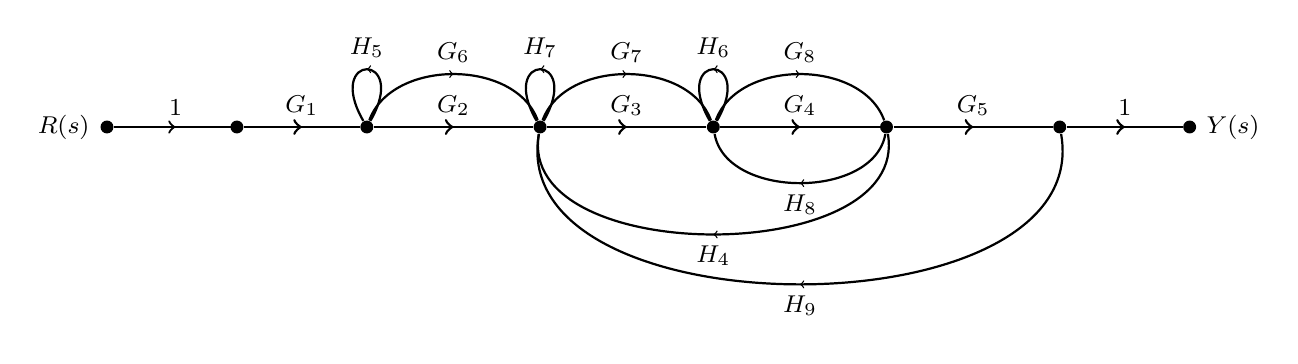
\begin{tikzpicture}[scale=1.1, transform shape, font=\footnotesize]
    % Nodes in forward G-series
    \node (Rtext) at (-1.5,0) {$R(s)$};
    \node[circle, fill=black, inner sep=1.5pt] (R) at (-1,0) {};
    \node[circle, fill=black, inner sep=1.5pt] (X) at (0.5,0) {};
    \node[circle, fill=black, inner sep=1.5pt] (X1) at (2,0) {};
    \node[circle, fill=black, inner sep=1.5pt] (X2) at (4,0) {};
    \node[circle, fill=black, inner sep=1.5pt] (X3) at (6,0) {};
    \node[circle, fill=black, inner sep=1.5pt] (X4) at (8,0) {};
    \node[circle, fill=black, inner sep=1.5pt] (X5) at (10,0) {};
    \node[circle, fill=black, inner sep=1.5pt] (Y)  at (11.5,0) {};
    \node (Ytext) at (12,0) {$Y(s)$};
    
    % Forward G-series
    \draw[thick, postaction={decorate, decoration={markings, mark=at position 0.5 with {\arrow[scale=1, fill=black]{>}}}}]
    (R) -- node[above] {$1$} (0.5,0);
    \draw[thick, postaction={decorate, decoration={markings, mark=at position 0.5 with {\arrow[scale=1.2]{>}}}}] (X) -- node[above] {$G_1$} (X1);
    \draw[thick, postaction={decorate, decoration={markings, mark=at position 0.5 with {\arrow[scale=1.2]{>}}}}] (X1) -- node[above] {$G_2$} (X2);
    \draw[thick, postaction={decorate, decoration={markings, mark=at position 0.5 with {\arrow[scale=1.2]{>}}}}] (X2) -- node[above] {$G_3$} (X3);
    \draw[thick, postaction={decorate, decoration={markings, mark=at position 0.5 with {\arrow[scale=1.2]{>}}}}] (X3) -- node[above] {$G_4$} (X4);
    \draw[thick, postaction={decorate, decoration={markings, mark=at position 0.5 with {\arrow[scale=1.2]{>}}}}] (X4) -- node[above] {$G_5$} (X5);
    \draw[thick, postaction={decorate, decoration={markings, mark=at position 0.5 with {\arrow[scale=1.2]{>}}}}] (X5) -- node[above] {$1$} (Y);    
    
    % H connections (loops)
    \draw[thick, midarrow] (X1) to[bend left=70] node[above] {$G_6$} (X2);
    \draw[thick, midarrow] (X2) to[bend left=70] node[above] {$G_7$} (X3);
    \draw[thick, midarrow] (X3) to[bend left=70] node[above] {$G_8$} (X4);
    
    % loop (Y back to X2)
    \draw[thick, midarrow] (X4) to[bend left=100] node[below] {$H_4$} (X2);
    
    % Self-loops with mid-arrow
    \draw[thick, midarrow] (X1) .. controls +(60:1cm) and +(120:1cm) .. node[above] {$H_5$} (X1);
    \draw[thick, midarrow] (X3) .. controls +(60:1cm) and +(120:1cm) .. node[above] {$H_6$} (X3);
    
    \draw[thick, midarrow] (X2) .. controls +(60:1cm) and +(120:1cm) .. node[above] {$H_7$} (X2); % X2 self-loop
    \draw[thick, midarrow] (X4) to[bend left=80] node[below] {$H_8$} (X3);
    \draw[thick, midarrow] (X5) to[bend left=100] node[below] {$H_9$} (X2);
    
\end{tikzpicture}
\end{figure}

\noindent\rule{\textwidth}{1pt}

\textbf{Given:} 
\[
G_1, G_2, G_3, G_4, G_5
\]
\[
R(s), \quad Y(s)
\]
\[
H_4 \text{ from } X_4 \text{ to } X_2,\; H_5 \text{ at } X_1,\; H_6 \text{ at } X_3
\]
\[
G_6, G_7, G_8
\]

\textbf{Required:} 
\[
(T(s) = \frac{Y(s)}{R(s)}
\]

\textbf{Solution:}

Forward Path:

\[
P_1 = 1 \cdot G_1 \cdot G_2 \cdot G_3 \cdot G_4 \cdot G_5 \cdot 1 
\]
\[
P_1 = G_1 G_2 G_3 G_4 G_5
\]

Loops:

\[
\begin{aligned}
L_1 &: \text{Self-loop at } X_1 \text{ with gain } H_5, \\
L_2 &: \text{Self-loop at } X_3 \text{ with gain } H_6, \\
L_3 &: \text{Loop from } X_4 \rightarrow X_2 \rightarrow X_3 \rightarrow X_4 \text{ with gain } H_4 G_3 G_8, \\
L_4 &: \text{Forward curved path loop } X_1 \rightarrow X_2 \rightarrow X_3 \rightarrow X_4 \text{ with gain } G_6 G_7 G_8
\end{aligned}
\]

Non-touching loops:
\[
L_1 \text{ and } L_2 \quad (\text{self-loops do not touch each other})
\]

Determinant \(\Delta\):
\[
\Delta = 1 - (L_1 + L_2 + L_3 + L_4) + (L_1 L_2) 
\]

\[
\Delta_1 = 1 - (\text{loops not touching } P_1)
\]

Transfer function using Mason's Gain Formula:

\[
T(s) = \frac{Y(s)}{R(s)} = \frac{P_1 \Delta_1}{\Delta}
\]

\[
\boxed{
T(s) = \frac{G_1 G_2 G_3 G_4 G_5 (1 - \text{loops not touching } P_1)}{1 - (L_1 + L_2 + L_3 + L_4) + L_1 L_2}
}
\]

% Problem 47
\newpage

\noindent\rule{\textwidth}{1pt}
\noindent\textbf{Problem 47} \hfill
\\ Using Mason's Rule, determine the transfer function \(T(s) = \frac{Y(s)}{R(s)}\) for the signal flow graph shown below.

\begin{figure}[h!]
\centering
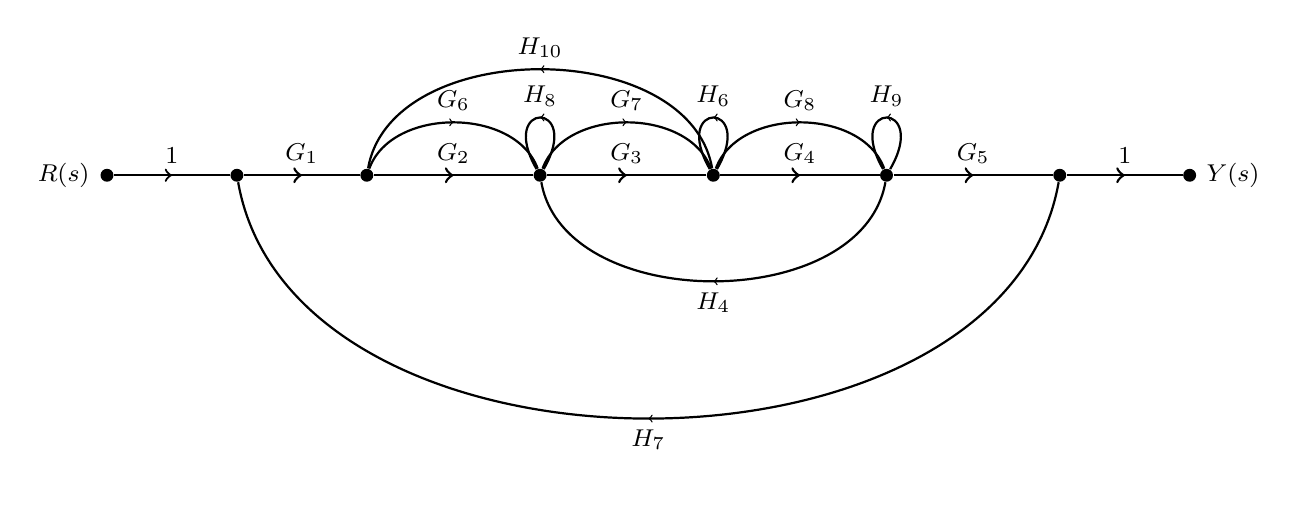
\begin{tikzpicture}[scale=1.1, transform shape, font=\footnotesize]
    % Nodes in a straight line (forward G-series)
    \node (Rtext) at (-1.5,0) {$R(s)$};
    \node[circle, fill=black, inner sep=1.5pt] (R) at (-1,0) {};
    \node[circle, fill=black, inner sep=1.5pt] (X) at (0.5,0) {};
    \node[circle, fill=black, inner sep=1.5pt] (X1) at (2,0) {};
    \node[circle, fill=black, inner sep=1.5pt] (X2) at (4,0) {};
    \node[circle, fill=black, inner sep=1.5pt] (X3) at (6,0) {};
    \node[circle, fill=black, inner sep=1.5pt] (X4) at (8,0) {};
    \node[circle, fill=black, inner sep=1.5pt] (X5) at (10,0) {};
    \node[circle, fill=black, inner sep=1.5pt] (Y)  at (11.5,0) {};
    \node (Ytext) at (12,0) {$Y(s)$};
    
    % Forward G-series
    \draw[thick, postaction={decorate, decoration={markings, mark=at position 0.5 with {\arrow[scale=1]{>}}}}] (R) -- node[above] {$1$} (X);
    \draw[thick, postaction={decorate, decoration={markings, mark=at position 0.5 with {\arrow[scale=1.2]{>}}}}] (X) -- node[above] {$G_1$} (X1);
    \draw[thick, postaction={decorate, decoration={markings, mark=at position 0.5 with {\arrow[scale=1.2]{>}}}}] (X1) -- node[above] {$G_2$} (X2);
    \draw[thick, postaction={decorate, decoration={markings, mark=at position 0.5 with {\arrow[scale=1.2]{>}}}}] (X2) -- node[above] {$G_3$} (X3);
    \draw[thick, postaction={decorate, decoration={markings, mark=at position 0.5 with {\arrow[scale=1.2]{>}}}}] (X3) -- node[above] {$G_4$} (X4);
    \draw[thick, postaction={decorate, decoration={markings, mark=at position 0.5 with {\arrow[scale=1.2]{>}}}}] (X4) -- node[above] {$G_5$} (X5);
    \draw[thick, postaction={decorate, decoration={markings, mark=at position 0.5 with {\arrow[scale=1.2]{>}}}}] (X5) -- node[above] {$1$} (Y);    
    
    % Curved forward paths
    \draw[thick, midarrow] (X1) to[bend left=70] node[above] {$G_6$} (X2);
    \draw[thick, midarrow] (X2) to[bend left=70] node[above] {$G_7$} (X3);
    \draw[thick, midarrow] (X3) to[bend left=70] node[above] {$G_8$} (X4);
    
    % Original loops with colors
    \draw[thick, midarrow] (X4) to[bend left=80] node[below] {$H_4$} (X2);
    \draw[thick, midarrow] (X3) .. controls +(60:1cm) and +(120:1cm) .. node[above] {$H_6$} (X3);
    \draw[thick, midarrow] (X5) to[bend left=80] node[below] {$H_7$} (X);

    % New loops
    \draw[thick, midarrow] (X2) .. controls +(60:1cm) and +(120:1cm) .. node[above] {$H_8$} (X2);
    \draw[thick, midarrow] (X4) .. controls +(60:1cm) and +(120:1cm) .. node[above] {$H_9$} (X4);
    \draw[thick, midarrow] (X3) to[bend right=80] node[above] {$H_{10}$} (X1);

\end{tikzpicture}
\end{figure}


\noindent\rule{\textwidth}{1pt}

\textbf{Given:}
\[
\text{Nodes: } R(s) \longrightarrow X \longrightarrow X_1 \longrightarrow X_2 \longrightarrow X_3 \longrightarrow X_4 \longrightarrow X_5 \longrightarrow Y(s)
\]
\[
\text{Forward path gains: } G_1,\; G_2,\; G_3,\; G_4,\; G_5
\]
\[
\text{Additional forward branches: } G_6: X_1 \to X_2,\; G_7: X_2 \to X_3,\; G_8: X_3 \to X_4
\]
\[
H_4 : X_4 \to X_2,
\]
\[
H_5 : X_1 \to X_2
\]
\[
H_6 : \text{self-loop at } X_3
\]
\[
H_7 : X_5 \to X
\]
\[
H_8 : \text{self-loop at } X_2
\]
\[
H_9 : \text{self-loop at } X_4
\]
\[
H_{10} : X_3 \to X_1
\]

\textbf{Required:} Find the overall transfer function
\[
T(s) = \frac{Y(s)}{R(s)}
\]

\textbf{Solution:}

Forward paths \(P_k\)
\[
P_{\text{total}} = G_1 \,(G_2 + G_6)\,(G_3 + G_7)\,(G_4 + G_8)\,G_5
\]
\[
P_{\text{total}} = G_1 \, S_2 \, S_3 \, S_4 \, G_5
\]

where we define
\[
S_2 = G_2 + G_6, \quad S_3 = G_3 + G_7, \quad S_4 = G_4 + G_8
\]

Individual loops \(L_i\)
\begin{align*}
L_1 &= H_6 \quad \text{(self-loop at } X_3 \text{)} \\
L_2 &= H_4 \times \text{gain from } X_2 \text{ to } X_4 = H_4 \, S_3 \, S_4 \\
L_3 &= H_7 \times \text{gain from } X \text{ to } X_5 = H_7 \, G_1 \, S_2 \, S_3 \, S_4 \, G_5 \\
L_4 &= H_8 \quad \text{(self-loop at } X_2 \text{)} \\
L_5 &= H_9 \quad \text{(self-loop at } X_4 \text{)} \\
L_6 &= H_{10} \times \text{gain from } X_1 \text{ to } X_3 = H_{10} \, S_2 \, S_3
\end{align*}

\newpage
Non-touching loops

\[\text{no non-touching loops exist}\]

Mason's determinant
\[
\Delta = 1 - \sum_{i=1}^{6} L_i
= 1 - (L_1 + L_2 + L_3 + L_4 + L_5 + L_6)
\]

\[
\Delta_k = 1 \quad \text{(for each forward path, since no non-touching loops)}
\]

By Mason's Gain Formula:
\[
T(s) = \frac{\sum_k P_k \Delta_k}{\Delta} = \frac{P_{\text{total}}}{\Delta}
\]

\[
\boxed{%
T(s) = \frac{G_1\,S_2\,S_3\,S_4\,G_5}
{\,1 - \Big(H_6 + H_4\,S_3\,S_4 + H_7\,G_1\,S_2\,S_3\,S_4\,G_5 + H_8 + H_9 + H_{10}\,S_2\,S_3 \Big)\,}
}
\]

% Problem 48
\newpage

\noindent\rule{\textwidth}{1pt}
\noindent\textbf{Problem 48} \hfill
\\ Using Mason's Rule, determine the transfer function \(T(s) = \frac{Y(s)}{R(s)}\) for the signal flow graph shown below.

\begin{figure}[h!]
\centering
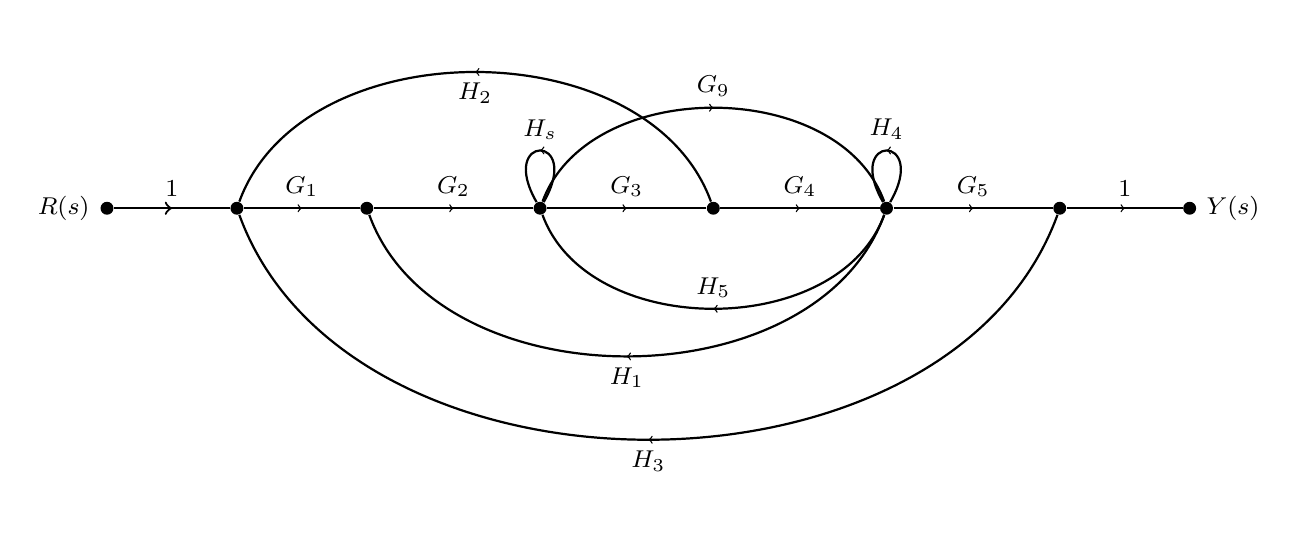
\begin{tikzpicture}[scale=1.1, transform shape, font=\footnotesize]

    % Nodes in forward G-series
    \node (Rtext) at (-1.5,0) {$R(s)$};
    \node[circle, fill=black, inner sep=1.5pt] (R) at (-1,0) {};
    \node[circle, fill=black, inner sep=1.5pt] (X) at (0.5,0) {};
    \node[circle, fill=black, inner sep=1.5pt] (X1) at (2,0) {};
    \node[circle, fill=black, inner sep=1.5pt] (X2) at (4,0) {};
    \node[circle, fill=black, inner sep=1.5pt] (X3) at (6,0) {};
    \node[circle, fill=black, inner sep=1.5pt] (X4) at (8,0) {};
    \node[circle, fill=black, inner sep=1.5pt] (X5) at (10,0) {};
    \node[circle, fill=black, inner sep=1.5pt] (Y)  at (11.5,0) {};
    \node (Ytext) at (12,0) {$Y(s)$};
    
    % Forward G-series 
    \draw[thick, postaction={decorate, decoration={markings, mark=at position 0.5 with {\arrow[scale=1, fill=black]{>}}}}] 
        (R) -- node[above] {$1$} (X);
    \draw[thick, midarrow] (X) -- node[above] {$G_1$} (X1);
    \draw[thick, midarrow] (X1) -- node[above] {$G_2$} (X2);
    \draw[thick, midarrow] (X2) -- node[above] {$G_3$} (X3);
    \draw[thick, midarrow] (X3) -- node[above] {$G_4$} (X4);
    \draw[thick, midarrow] (X4) -- node[above] {$G_5$} (X5);
    \draw[thick, midarrow] (X5) -- node[above] {$1$} (Y);    
    
    % Extra forward branch: X2 -> X4 (G9)
    \draw[thick, midarrow] (X2) to[bend left=70] node[above] {$G_9$} (X4);
    
    % Feedback loops
    \draw[thick, midarrow] (X4) to[bend left=70] node[below] {$H_1$} (X1);
    \draw[thick, midarrow] (X3) to[bend right=70] node[below] {$H_2$} (X);
    \draw[thick, midarrow] (X2) .. controls +(60:1cm) and +(120:1cm) .. node[above] {$H_s$} (X2);
    \draw[thick, midarrow] (X5) to[bend left=70] node[below] {$H_3$} (X);
    \draw[thick, midarrow] (X4) .. controls +(60:1cm) and +(120:1cm) .. node[above] {$H_4$} (X4);
    \draw[thick, midarrow] (X4) to[bend left=70] node[above] {$H_5$} (X2);

\end{tikzpicture}
\end{figure}

\noindent\rule{\textwidth}{1pt}

\textbf{Given:}
\[
\text{Nodes: } R(s)\longrightarrow X \longrightarrow X_1 \longrightarrow X_2 \longrightarrow X_3 \longrightarrow X_4 \longrightarrow X_5 \longrightarrow Y(s)
\]
\[
\text{Main forward gains: } G_1, G_2, G_3, G_4, G_5
\]
\[
\text{Extra forward branch: } G_9: X_2 \to X_4
\]
\[
H_1: X_4 \to X_1 \quad \text{(feedback loop)}
\]
\[
H_2: X_3 \to X \quad \text{(feedback loop)}
\]
\[
H_3: X_5 \to X \quad \text{(feedback loop)}
\]
\[
H_s: \text{self-loop at } X_2
\]
\[
H_4: \text{self-loop at } X_4
\]
\[
H_5: X_4 \to X_2 \quad \text{(feedback loop)}
\]


\textbf{Required:}
\[
\text{Find } T(s)=\frac{Y(s)}{R(s)} \text{ using Mason's Gain Formula.}
\]

\textbf{Solution:}

Forward Paths

\[
P_1: R\to X\to X_1\to X_2\to X_3\to X_4\to X_5\to Y
\]
\[
P_1 = G_1 G_2 G_3 G_4 G_5
\]

\[
P_2: R\to X\to X_1\to X_2 \xrightarrow{G_9} X_4 \to X_5 \to Y
\]
\[
P_2 = G_1 G_2 G_9 G_5
\]

\[
\sum_k P_k = P_1 + P_2 = G_1 G_2 (G_3 G_4 G_5 + G_9 G_5) 
\]
\[
\sum_k P_k = G_1 G_2 S G_5
\]

\[
\text{where } S := G_3 G_4 + G_9 \quad (\text{gain from } X_2 \text{ to } X_4)
\]

Individual Loops

\[
L_s = H_s \quad \text{(self-loop at } X_2)
\]

\[
L_1 = H_1 \cdot \text{(gain from } X_1 \text{ to } X_4) = H_1 G_2 S
\]

\[
L_2 = H_2 \cdot \text{(gain from } X \text{ to } X_3) = H_2 G_1 G_2 G_3
\]

\[
L_3 = H_3 \cdot \text{(gain from } X \text{ to } X_5) = H_3 G_1 G_2 S G_5
\]

\[
L_4 = H_4 \quad \text{(self-loop at } X_4)
\]

\[
L_5 = H_5 \cdot \text{(gain from } X_2 \text{ to } X_4) = H_5 S
\]

Non-touching loops
\[\text{no non-touching loop pairs}\]

Mason's Determinant \(\Delta\) and \(\Delta_k\)
\[
\Delta = 1 - \sum_i L_i + \sum_{\text{non-touching pairs}} L_i L_j - \dots
\]

Since no non-touching pairs:

\[
\Delta = 1 - (L_s + L_1 + L_2 + L_3 + L_4 + L_5)
\]

\[
\Delta = 1 - \Big( H_s + H_1 G_2 S + H_2 G_1 G_2 G_3 + H_3 G_1 G_2 S G_5 + H_4 + H_5 S \Big)
\]

\[
\Delta_1 = 1 \quad (\text{loops touching } P_1 \text{ removed})
\]

\[
\Delta_2 = 1 - (L_2) = 1 - H_2 G_1 G_2 G_3
\]

Mason's Gain Formula

\[
T(s) = \frac{\sum_k P_k \Delta_k}{\Delta} = \frac{P_1 \Delta_1 + P_2 \Delta_2}{\Delta}
\]

\[
T(s) = \frac{G_1 G_2 G_3 G_4 G_5 \cdot 1 + G_1 G_2 G_9 G_5 \cdot (1 - H_2 G_1 G_2 G_3)}
{1 - (H_s + H_1 G_2 S + H_2 G_1 G_2 G_3 + H_3 G_1 G_2 S G_5 + H_4 + H_5 S)}
\]

\[
\boxed{
T(s) = \frac{G_1 G_2 G_3 G_4 G_5 + G_1 G_2 G_9 G_5 (1 - H_2 G_1 G_2 G_3)}
{1 - \big(H_s + H_1 G_2 S + H_2 G_1 G_2 G_3 + H_3 G_1 G_2 S G_5 + H_4 + H_5 S\big)}
}
\]

% Problem 49
\newpage

\noindent\rule{\textwidth}{1pt}
\noindent\textbf{Problem 49} \hfill
\\ Using Mason's Rule, determine the transfer function \(T(s) = \frac{Y(s)}{R(s)}\) for the signal flow graph shown below.

\begin{figure}[h!]
\centering
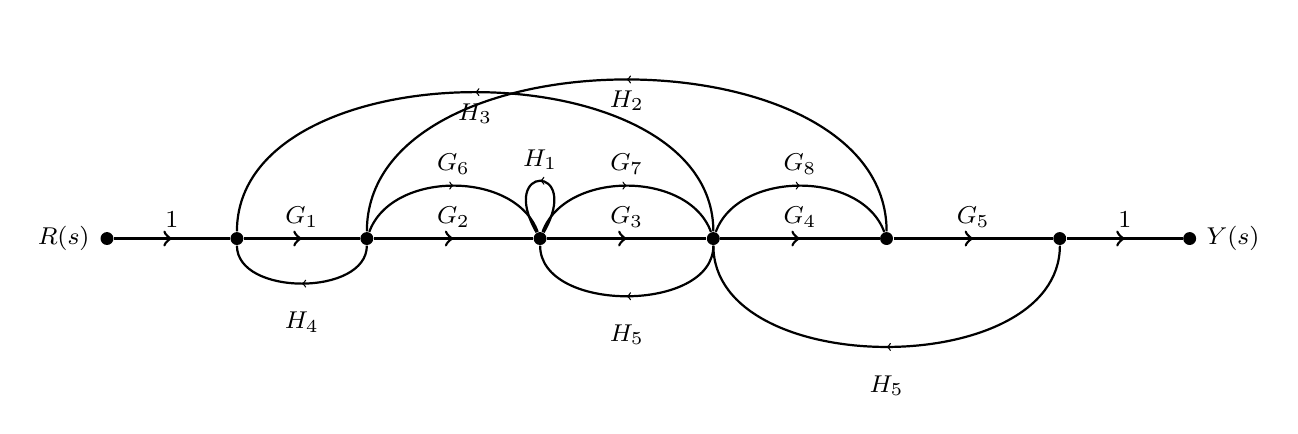
\begin{tikzpicture}[scale=1.1, transform shape, font=\footnotesize]
    
    % Nodes in a straight line
    \node (Rtext) at (-1.5,0) {$R(s)$};
    \node[circle, fill=black, inner sep=1.5pt] (R) at (-1,0) {};
    \node[circle, fill=black, inner sep=1.5pt] (X) at (0.5,0) {};
    \node[circle, fill=black, inner sep=1.5pt] (X1) at (2,0) {};
    \node[circle, fill=black, inner sep=1.5pt] (X2) at (4,0) {};
    \node[circle, fill=black, inner sep=1.5pt] (X3) at (6,0) {};
    \node[circle, fill=black, inner sep=1.5pt] (X4) at (8,0) {};
    \node[circle, fill=black, inner sep=1.5pt] (X5) at (10,0) {};
    \node[circle, fill=black, inner sep=1.5pt] (Y)  at (11.5,0) {};
    \node (Ytext) at (12,0) {$Y(s)$};
    
    % Forward G-series
    \draw[thick, postaction={decorate, decoration={markings, mark=at position 0.5 with {\arrow[scale=1.2]{>}}}}] (R) -- node[above] {$1$} (X);
    \draw[thick, postaction={decorate, decoration={markings, mark=at position 0.5 with {\arrow[scale=1.2]{>}}}}] (X) -- node[above] {$G_1$} (X1);
    \draw[thick, postaction={decorate, decoration={markings, mark=at position 0.5 with {\arrow[scale=1.2]{>}}}}] (X1) -- node[above] {$G_2$} (X2);
    \draw[thick, postaction={decorate, decoration={markings, mark=at position 0.5 with {\arrow[scale=1.2]{>}}}}] (X2) -- node[above] {$G_3$} (X3);
    \draw[thick, postaction={decorate, decoration={markings, mark=at position 0.5 with {\arrow[scale=1.2]{>}}}}] (X3) -- node[above] {$G_4$} (X4);
    \draw[thick, postaction={decorate, decoration={markings, mark=at position 0.5 with {\arrow[scale=1.2]{>}}}}] (X4) -- node[above] {$G_5$} (X5);
    \draw[thick, postaction={decorate, decoration={markings, mark=at position 0.5 with {\arrow[scale=1.2]{>}}}}] (X5) -- node[above] {$1$} (Y);    
    
    % G connections 
    \draw[thick, midarrow] (X1) to[bend left=70] node[above] {$G_6$} (X2);
    \draw[thick, midarrow] (X2) to[bend left=70] node[above] {$G_7$} (X3);
    \draw[thick, midarrow] (X3) to[bend left=70] node[above] {$G_8$} (X4);
    
    % Self-loop on X2
    \draw[thick, midarrow] (X2) .. controls +(60:1cm) and +(120:1cm) .. node[above] {$H_1$} (X2);
    
    % Feedback loops
    \draw[thick, midarrow] (X4) to[bend right=90] node[below] {$H_2$} (X1);  
    \draw[thick, midarrow] (X3) to[bend right=90] node[below] {$H_3$} (X);   
    
    \draw[thick, midarrow] (X1) to[out=-90,in=-90] node[below=0.2cm] {$H_4$} (X);
    \draw[thick, midarrow] (X5) to[out=-90,in=-90] node[below=0.2cm] {$H_5$} (X3);
    \draw[thick, midarrow] (X3) to[out=-90,in=-90] node[below=0.2cm] {$H_5$} (X2);
    
\end{tikzpicture}
\end{figure}

\noindent\rule{\textwidth}{1pt}

\textbf{Given:}
\[
\text{Signal flow graph nodes: } R(s), X, X_1, X_2, X_3, X_4, X_5, Y(s)
\]
\[
\text{Forward path gains: } G_1, G_2, G_3, G_4, G_5, G_6, G_7, G_8
\]
\[
\text{Feedback loops:} 
\]
\[
H_1: \text{self-loop at } X_2
\]
\[
H_2: X_4 \to X_1
\]
\[
H_3: X_3 \to X
\]
\[
H_4: X_1 \to X \; (\text{below G}_1)
\]
\[
H_5: X_5 \to X_3
\]
\[
H_6: X_3 \to X_2 \; (\text{optional additional feedback})
\]

\textbf{Required:}
\[
\text{Compute the transfer function } T(s) = \frac{Y(s)}{R(s)} \text{ symbolically.}
\]

\textbf{Solution:}

Forward Paths
\[
P_1: R \to X \to X_1 \to X_2 \to X_3 \to X_4 \to X_5 \to Y
\]
\[
P_1 = G_1 G_2 G_3 G_4 G_5
\]
\[
P_2: R \to X \to X_1 \to X_2 \to X_3 \to X_4 \to X_5 \to Y 
\]
\[
P_3: R \to X \to X_1 \to X_3 \to X_4 \to X_5 \to Y
\]
\[
P_3 = G_1 G_6 G_4 G_5
\]
\[
P_4: R \to X \to X_1 \to X_2 \to X_5 \to Y
\]
\[
P_4 = G_1 G_2 G_7 G_5
\]

Individual Loops

\[
\begin{aligned}
L_1 &= H_1 \quad (\text{self-loop at } X_2)\\
L_2 &= H_2 \cdot (\text{path } X_1 \to X_2 \to X_3 \to X_4) = H_2 G_2 G_3 G_4\\
L_3 &= H_3 \cdot (\text{path } X \to X_1 \to X_2 \to X_3) = H_3 G_1 G_2 G_3\\
L_4 &= H_4 \quad (\text{loop from } X_1 \text{ to } X \text{ below } G_1)\\
L_5 &= H_5 \cdot (\text{path } X_5 \to X_4 \to X_3) = H_5 G_4 G_3\\
L_6 &= H_6 \cdot (\text{path } X_3 \to X_2) = H_6 G_3
\end{aligned}
\]

Non-touching Loops
\[
\text{no non-touching loop pairs exist.}
\]

Mason's Gain Formula Determinant

\[
\Delta = 1 - \sum_i L_i + \sum_{i<j} (L_i L_j) - \dots
\]

Since no non-touching loops exist:

\[
\Delta = 1 - (L_1 + L_2 + L_3 + L_4 + L_5 + L_6)
\]

\[
\Delta_k = 1 \quad \text{for all forward paths } P_k
\]

Mason's Gain Formula

\[
T(s) = \frac{\sum_k P_k \Delta_k}{\Delta} = \frac{P_1 + P_2 + P_3 + P_4}{1 - (L_1 + L_2 + L_3 + L_4 + L_5 + L_6)}
\]

\[
\boxed{
T(s) = \frac{
G_1 G_2 G_3 G_4 G_5 + G_1 G_6 G_4 G_5 + G_1 G_2 G_7 G_5
}{
1 - \big(H_1 + H_2 G_2 G_3 G_4 + H_3 G_1 G_2 G_3 + H_4 + H_5 G_4 G_3 + H_6 G_3 \big)
}
}
\]

% Problem 50
\newpage

\noindent\rule{\textwidth}{1pt}
\noindent\textbf{Problem 50} \hfill
\\ Using Mason's Rule, determine the transfer function \(T(s) = \frac{Y(s)}{R(s)}\) for the signal flow graph shown below.

\begin{figure}[h!]
\centering
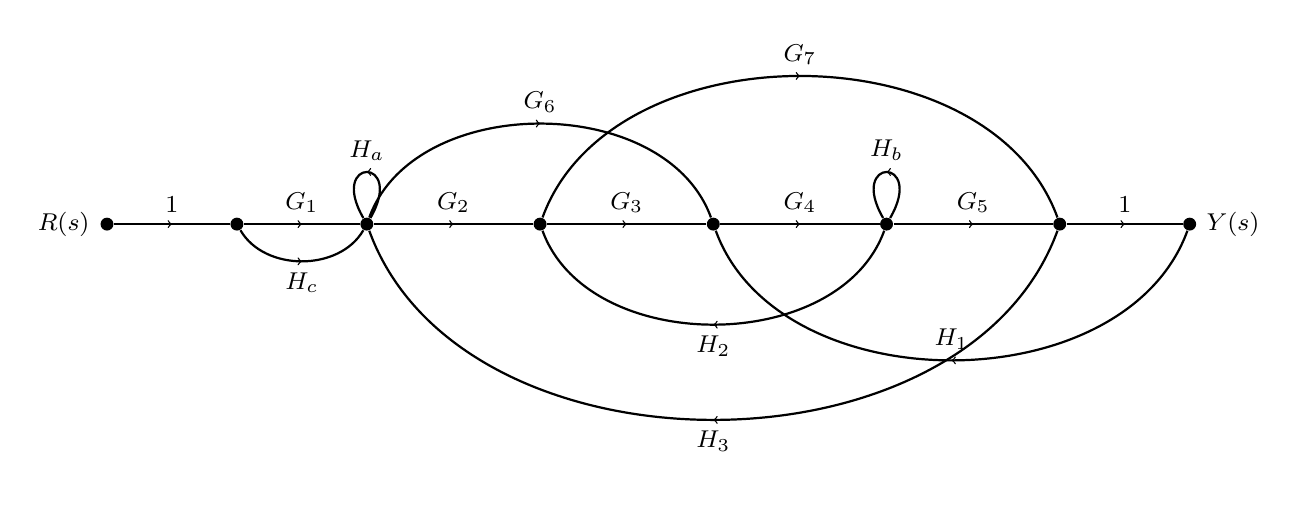
\begin{tikzpicture}[scale=1.1, transform shape, font=\footnotesize]
    
    % Nodes
    \node (Rtext) at (-1.5,0) {$R(s)$};
    \node[circle, fill=black, inner sep=1.5pt] (R) at (-1,0) {};
    \node[circle, fill=black, inner sep=1.5pt] (X) at (0.5,0) {};
    \node[circle, fill=black, inner sep=1.5pt] (X1) at (2,0) {};
    \node[circle, fill=black, inner sep=1.5pt] (X2) at (4,0) {};
    \node[circle, fill=black, inner sep=1.5pt] (X3) at (6,0) {};
    \node[circle, fill=black, inner sep=1.5pt] (X4) at (8,0) {};
    \node[circle, fill=black, inner sep=1.5pt] (X5) at (10,0) {};
    \node[circle, fill=black, inner sep=1.5pt] (Y)  at (11.5,0) {};
    \node (Ytext) at (12,0) {$Y(s)$};
    
    % Forward G-series
    \draw[thick, midarrow] (R) -- node[above] {$1$} (X);
    \draw[thick, midarrow] (X) -- node[above] {$G_1$} (X1);
    \draw[thick, midarrow] (X1) -- node[above] {$G_2$} (X2);
    \draw[thick, midarrow] (X2) -- node[above] {$G_3$} (X3);
    \draw[thick, midarrow] (X3) -- node[above] {$G_4$} (X4);
    \draw[thick, midarrow] (X4) -- node[above] {$G_5$} (X5);
    \draw[thick, midarrow] (X5) -- node[above] {$1$} (Y);
    
    % Feed-across branches
    \draw[thick, midarrow] (X1) to[bend left=70] node[above] {$G_6$} (X3);
    \draw[thick, midarrow] (X2) to[bend left=70] node[above] {$G_7$} (X5);
    
    % Feedback loops
    \draw[thick, midarrow] (Y) to[bend left=70] node[above] {$H_1$} (X3);    \draw[thick, midarrow] (X4) to[bend left=70] node[below] {$H_2$} (X2);  
    \draw[thick, midarrow] (X5) to[bend left=70] node[below] {$H_3$} (X1);  
    \draw[thick, midarrow] (X) to[bend right=60] node[below] {$H_c$} (X1);  
    
    % Self-loops
    \draw[thick, midarrow] (X1) .. controls +(60:0.9cm) and +(120:0.9cm) .. node[above] {$H_a$} (X1);
    \draw[thick, midarrow] (X4) .. controls +(60:0.9cm) and +(120:0.9cm) .. node[above] {$H_b$} (X4);
    
\end{tikzpicture}
\end{figure}


\noindent\rule{\textwidth}{1pt}

\textbf{Given:}
\[
\text{Signal flow graph nodes: } R(s), X, X_1, X_2, X_3, X_4, X_5, Y(s)
\]
\[
\text{Forward path gains: } G_1, G_2, G_3, G_4, G_5, G_6, G_7, G_8, G_9
\]
\[
\text{Feedback loops: } H_1: X_4 \to X_1
\]
\[
H_2: X_3 \to X
\]
\[
H_3: X_5 \to X
\]
\[
H_5: X_1 \to X_2
\]
\[
H_6: \text{self-loop at } X_3
\]
\[
H_7: X_5 \to X
\]

\textbf{Required:}
\[
\text{Compute the transfer function } T(s) = \frac{Y(s)}{R(s)} \text{ symbolically} \\[1mm]
\]

\textbf{Solution:}

Forward Paths

\[
P_1: R \to X \to X_1 \to X_2 \to X_3 \to X_4 \to X_5 \to Y
\]
\[
P_1 = G_1 G_2 G_3 G_4 G_5
\]
\[
P_2: R \to X \to X_1 \to X_3 \to X_4 \to X_5 \to Y \quad (\text{using } G_6)
\]
\[
P_2 = G_1 G_6 G_4 G_5
\]
\[
P_3: R \to X \to X_1 \to X_2 \to X_5 \to Y \quad (\text{using } G_7)
\]
\[
P_3 = G_1 G_2 G_7 G_5
\]

\textbf{Individual Loops:}
\[
L_1 = H_a \quad (\text{self-loop at } X_1)
\]
\[
L_2 = H_b \quad (\text{self-loop at } X_4)
\]
\[
L_3 = H_1 \cdot (\text{path } X_3 \to X_4 \to X_5 \to Y \to X_1) = H_1 G_4 G_5
\]
\[
L_4 = H_2 \cdot (\text{path } X \to X_1 \to X_2 \to X_3) = H_2 G_1 G_2 G_3
\]
\[
L_5 = H_3 \cdot (\text{path } X_1 \to X_2 \to X_3 \to X_4 \to X_5) = H_3 G_2 G_3 G_4 G_5
\]
\[
L_6 = H_5 \cdot (\text{path } X_2 \to X_3 \to X_4 \to X_5) = H_5 G_3 G_4 G_5
\]

\newpage
Non-Touching Loops

\[
L_1 \text{ touches all other loops via } X_1 \Rightarrow \text{no non-touching pairs including } L_1
\]
\[
L_2 \text{ touches all other loops via } X_4 \Rightarrow \text{no non-touching pairs including } L_2
\]
\[
L_3 \text{ touches } L_4 \text{ and } L_5 \text{ via } X_3,X_4,X_5
\]
\[
L_4 \text{ touches } L_5 \text{ via } X_2,X_3,X_4
\]
\[
\text{Hence: no non-touching loop pairs exist.}
\]

Mason's Gain Formula determinant:

\[
\Delta = 1 - \sum L_i + \sum (\text{product of non-touching loops}) - \dots
\]
\[
\Delta = 1 - (L_1 + L_2 + L_3 + L_4 + L_5)
\]
\[
\Delta_k = 1 \quad (\text{since no non-touching loops for any forward path})
\]

Mason's Gain Formula

\[
T(s) = \frac{\sum_k P_k \Delta_k}{\Delta}
\]
\[
T(s) = \frac{P_1 + P_2 + P_3}{1 - (L_1 + L_2 + L_3 + L_4 + L_5)}
\]
\[
\boxed{
T(s) = \frac{G_1 G_2 G_3 G_4 G_5 + G_1 G_6 G_4 G_5 + G_1 G_2 G_7 G_5}{1 - (H_a + H_b + H_1 G_4 G_5 + H_2 G_1 G_2 G_3 + H_3 G_2 G_3 G_4 G_5)}
}
\]